% Provenance (never printed): see sources/outline_sources.md (Year 2: the solar nebula
% and the condensation sequence; planetesimals and embryos; chondrites, achondrites and
% irons; the age of the Solar System; differentiation of planets). Curves from
% figdata/bachelor-2/nebula.py, condensation.py, al26.py, meteorites.py; exercise and
% problem values in the Book 4 scratch calculator calc/ch02.py.
\chapter{行星形成与陨石}\label{ch:b2:planet-formation-meteorites}

每年约有一万五千吨来自太空的尘埃进入地球
大气层，其中大部分会烧毁或沉降为微观球粒，而偶尔
会有拳头大小的石块伴随火球与音爆坠落。
这些石块大多是小行星的碎片，许多几乎未曾改变
自形成以来的样子。切开并抛光一块，可见毫米级的
曾经熔融的岩石小珠、白色不规则的钙铝
矿物颗粒、金属薄片，它们都嵌在深色细粒胶结物中。白色
颗粒是太阳系中最古老的固体：铅同位素测定其年龄为
45.67 亿年。另一把“时钟”是一种早已消失的放射性铝同位素的衰变，
它可相对于前者测定其他组分的年龄，
误差在百万年的几分之一以内。本章追踪上一章中的盘，
讲述它如何演化为行星：哪些固体从冷却的气体中凝结，
以及在何处凝结；尘埃如何长成千米级的天体，再
进而形成行星；\omterm{def:b2:planet-formation-meteorites:fall-find}{陨石}是什么，它们如何测定这些事件的年代，以及为什么
一些最早的天体熔化并长出了铁质地核，而另一些
则保持了形成时的样子。
% ledger: rojas21:flux, lugaro:cai, gail:meteorites

\begin{recall}
年轻恒星周围环绕着\omterm{def:b2:ism-star-formation:disc}{原行星盘}，这些盘会在
数百万年内消失；距恒星 $r$ 处的尘粒受星光照射，
若恒星光度为 $L$，其平衡温度为 $T = \bigl(L/(16\pi\sigma r^2)\bigr)^{1/4}$
（见\cref{ch:b2:ism-star-formation}）。小行星是太阳系中较小的岩质或金属天体，
大多数位于火星与木星之间的轨道上（见本科一年级
分册）。放射性原子核以单位时间内的概率 $\lambda$ 衰变，
其规律为 $N = N_0 e^{-\lambda t}$；半衰期为 $\ln 2/\lambda$，平均
寿命为 $\tau = 1/\lambda$（见物理各册）。在封闭系统中，同源样品的
母体与子体比值各不相同，则其数据点位于一条直线上，称为等时线，其
斜率给出年龄，截距为初始比值（见本科一年级分册）。
对质量为 $m$、比热容为 $c$ 的物体加热，使其升温 $\Delta T$，所需
能量为 $mc\,\Delta T$（见物理各册）。
\end{recall}

\section{太阳星云}

\begin{definition}[太阳星云]\label{def:b2:planet-formation-meteorites:nebula}
称\emph{太阳星云}\index{太阳星云}为由气体和尘埃组成的\omterm{def:b2:ism-star-formation:disc}{原行星盘}，
它环绕年轻的太阳，行星及其卫星、小行星和彗星
都由它形成。
\end{definition}

这个盘含有多少物质？一个下限来自行星本身。
为每颗行星补充足够的氢和氦，使其成分与
太阳相同，再把所得物质摊铺在以其轨道为中心的圆环上，于是面密度
（即盘中单位面积的质量）随离太阳距离的增大而减小。
这一重建称为\emph{最小质量
太阳星云}\index{最小质量太阳星云}。在一个广泛使用的版本中，
气体的面密度为
\[
  \Sigma_g = \qty{2200}{g.cm^{-2}}\left(\frac{r}{\qty{1}{au}}\right)^{-3/2},
\]
而固体的面密度为 $\Sigma_p = \qty{33}{g.cm^{-2}}\,Z_{\mathrm{rel}}\,
(r/\qty{1}{au})^{-3/2}$，其中 $Z_{\mathrm{rel}}$ 为
可凝结物质中实际呈固态的比例：仅岩石和金属凝结时为 $0.33$，
水冰也加入后约为 $0.78$，甲烷凝固之处以外则为 $1$。
这些数值并不确定：木星的重元素含量
只能确定到相差四倍之内，而行星未必
在其现在所处的轨道上形成。
% ledger: cy10:mmsn

\begin{proposition}[盘的质量]\label{prop:b2:planet-formation-meteorites:disc-mass}
面密度为 $\Sigma(r) = \Sigma_1 (r/r_1)^{-3/2}$ 的盘，
在半径 $R$ 以内所含的质量为
\[
  M(R) = 4\pi\Sigma_1 r_1^2 \left(\frac{R}{r_1}\right)^{1/2}.
\]
质量主要集中在外侧：半径加倍会使质量
增加 \qty{41}{\percent}。
\end{proposition}

\begin{proof}
半径为 $r$、宽为 $\mathrm dr$ 的圆环面积为 $2\pi r\,\mathrm dr$，于是
\[
  M(R) = \int_0^R 2\pi r\,\Sigma_1 \left(\frac{r}{r_1}\right)^{-3/2}\mathrm dr
       = 2\pi\Sigma_1 r_1^{3/2}\int_0^R r^{-1/2}\,\mathrm dr
       = 4\pi\Sigma_1 r_1^{3/2} R^{1/2},
\]
这即所求公式；积分在 $r = 0$ 处收敛。将 $R$ 加倍
使 $M$ 变为原来的 $\sqrt 2 = 1.41$ 倍。
\end{proof}

取 $\Sigma_1 = \qty{2.2e4}{kg.m^{-2}}$，$r_1 = \qty{1}{au}$，则最小质量
\omterm{def:b2:planet-formation-meteorites:nebula}{太阳星云}在 \qty{100}{au} 以内的质量为 $0.03$ 个太阳质量（见\cref{exo:b2:planet-formation-meteorites:5}）。这些
盘在年龄约百万年的恒星周围被观测到，并由其尘埃的毫米波辐射估算质量，
其质量为 \numrange{0.001}{0.1} 个太阳质量：最小质量\omterm{def:b2:planet-formation-meteorites:nebula}{太阳星云}
恰好位于这一范围之中。
% ledger: cy10:mmsn

这一质量中几乎全部是永远不会凝结的气体。太阳诞生时的
质量分数为：氢 $X_0 = 0.711$，氦 $Y_0 = 0.274$，而
所有更重元素合计仅为 $Z_0 = 0.0149$。将具有这一成分的气体冷却，
直到一切能够凝固的物质都已凝固，此时只有
\qty{1.5}{\percent} 的质量转化为固体：岩石和金属占 \qty{0.49}{\percent}，
另有 \qty{1.0}{\percent} 为水、甲烷和氨的冰，其中仅水冰就占
\qty{0.57}{\percent}。所有岩质行星以及巨行星的核心，
都是由这一小部分物质构成的。
% ledger: lodders:protosolar, lodders:condensates

盘的温度决定了何处呈何种固态。仅由恒星加热的盘，即
\emph{被动}盘，其表面较热，尘粒直接受到恒星照射，
（\cref{ch:b2:ism-star-formation}中的命题），而其中面则
冷得多，只接收表层尘粒再辐射出的红外线。
对于质量为一个太阳质量的年轻恒星，此类盘的模型
给出其中面温度为
\[
  T = \qty{120}{K}\left(\frac{r}{\qty{1}{au}}\right)^{-3/7}.
\]
盘中气体的吸积释放引力能，使
中面升温，尤其在早期和靠近恒星处（见下图）。
% ledger: cy10:passive

\begin{omfigure}
\begin{tikzpicture}
\begin{axis}[omrecord, width=0.82\linewidth, height=6.2cm, xmode=log, ymode=log,
  xmin=0.1, xmax=100, ymin=10, ymax=1000,
  xlabel={离恒星的距离 $r$ (au)}, ylabel={温度 (K)},
  tick label style={font=\scriptsize}, label style={font=\small},
  legend pos=north east, legend style={font=\scriptsize, draw=black!30}]
\addplot[thick, red!70!black] table[x=r_au, y=T_grain] {figdata/out/bachelor-2-nebula-temp.dat};
\addlegendentry{受直接星光照射的尘粒}
\addplot[thick, blue!70!black] table[x=r_au, y=T_mid] {figdata/out/bachelor-2-nebula-temp.dat};
\addlegendentry{被动盘的中面}
\addplot[black!50, densely dashed, domain=0.1:100, samples=2] {182};
\addplot[black!50, densely dashed, domain=0.1:100, samples=2] {41};
\node[font=\scriptsize, anchor=south east] at (axis cs:95,182) {水冰，\qty{182}{K}};
\node[font=\scriptsize, anchor=north west] at (axis cs:0.46,41) {甲烷冰，\qty{41}{K}};
\draw[blue!70!black, -latex] (axis cs:0.38,25) -- (axis cs:0.38,175);
\node[font=\scriptsize, blue!70!black, anchor=north] at (axis cs:0.38,25) {\qty{0.4}{au}};
\draw[red!70!black, -latex] (axis cs:2.34,25) -- (axis cs:2.34,175);
\node[font=\scriptsize, red!70!black, anchor=north] at (axis cs:2.34,25) {\qty{2.3}{au}};
\end{axis}
\end{tikzpicture}

\par\smallskip{\small 光度为一个太阳光度的恒星周围盘的两种温度。
红色：直接受星光照射的黑色尘粒（\cref{ch:b2:ism-star-formation}）。蓝色：
围绕年轻太阳质量恒星的被动盘中面，受遮蔽而不受直接光照。
水冰在\qty{182}{K}以下稳定：箭头标出各曲线
与该线相交的位置。真实的\omterm{def:b2:planet-formation-meteorites:snow-line}{雪线}位于这些界限之间，并随盘的演化而移动。
数据来源：Chiang and Youdin (2010)；Lodders (2003)。}
% ledger: cy10:passive, lodders:phases, cy10:mmsn, sun:L, const:sigma
\end{omfigure}

\section{凝聚序列}

设想星云中靠近年轻太阳的气体足够热，使每种元素都呈蒸气状态，
并使其缓慢冷却，以保持气体与固体处于化学平衡。
随着温度下降，每种元素
依次离开气体进入固体，或以自身构成的化合物形式，
或溶解于已经形成的固体之中。

\begin{definition}[凝聚温度，凝聚序列]
\label{def:b2:planet-formation-meteorites:condensation}
在给定成分与压强的冷却气体中，元素的\emph{凝聚温度}\index{凝聚温度}
是指其在化学平衡下有一半转入固体时的温度（即
\emph{50\% 凝聚温度}；元素出现第一个固相时的温度
称为\emph{出现温度}）。\emph{凝聚序列}\index{凝聚序列}
是指
随气体冷却，各元素及其固体化合物
依次出现的顺序。
\end{definition}

太阳成分气体的计算取总压强为
$10^{-4}$ bar，接近 \qty{1}{au} 处星云的典型值。最先出现的固体为
铝和钙的氧化物（见下表），约在
\qty{1700}{K}下形成；造岩物质的主体，硅酸镁与
金属铁，在\qty{1350}{K}附近凝结；硫化铁要等到
\qty{704}{K}，水冰则要到\qty{182}{K}才出现。
% ledger: lodders:phases

\begin{table}[h]
\centering
\small
\begin{tabular}{lll}
\hline
固体 & 化学式 & 出现温度 (K)\\
\hline
刚玉 & \ce{Al2O3} & 1677\\
黑柏石 & \ce{CaAl12O19} & 1659\\
钙钛矿 & \ce{CaTiO3} & 1593\\
尖晶石 & \ce{MgAl2O4} & 1397\\
铁镍金属 & \ce{Fe}，含 \ce{Ni}、\ce{Co}、\ce{Cr} & 1357\\
镁橄榄石 & \ce{Mg2SiO4} & 1354\\
磷铁镍矿 & \ce{Fe3P} & 1248\\
陨硫铁 & \ce{FeS} & 704\\
磁铁矿 & \ce{Fe3O4} & 371\\
水冰 & \ce{H2O} & 182\\
氨水合物 & \ce{NH3.H2O} & 131\\
甲烷笼形水合物 & \ce{CH4.7H2O} & 78\\
\hline
\end{tabular}
\caption{太阳系成分气体在
$10^{-4}$ bar 压强下的\omterm{def:b2:planet-formation-meteorites:condensation}{凝聚序列}：各固体首次出现的温度。钠和
钾进入长石；镍、钴和铬溶解于金属中。
数据来源：Lodders (2003)。}
\label{tab:b2:planet-formation-meteorites:sequence}
% ledger: lodders:phases
\end{table}

依据 50\% \omterm{def:b2:planet-formation-meteorites:condensation}{凝聚温度}，可将元素按
挥发性分为若干组（见下图）。凝结温度高于镁、硅和
铁的元素称为\emph{难熔}的，低于它们者称为\emph{挥发性}的。
Lodders 又将两类各自再细分：超难熔元素，即
高于\qty{1650}{K}者，包括铝、锆、重稀土元素以及
金属锇、铼和钨；高度难熔元素
（\qtyrange{1500}{1650}{K}）包括钙和钛；难熔元素
（\qtyrange{1360}{1500}{K}）包括锶、钡、钒和铂；
\emph{常见}
元素镁、硅和铁在\num{1290}与
\qty{1360}{K}之间凝结，连同镍、钴和铬；中等挥发性
元素，包括钠、钾、磷、铜、锌和
铅，凝结温度介于\qty{1290}{K}与陨硫铁的出现温度
\qty{704}{K}之间；挥发性元素中，包括硫、镉和铊，
凝结温度介于\num{704}与\qty{371}{K}之间；高度挥发性元素，
即碳、氮、以冰形式存在的氧、稀有气体和汞，凝结温度更低。
% ledger: lodders:groups, lodders:tc-table, lodders:tc-more

\begin{omfigure}
\begin{tikzpicture}
\begin{axis}[width=0.86\linewidth, height=10.5cm, xbar, bar width=4.2pt, bar shift=0pt,
  xmin=0, xmax=1950, ymin=0.3, ymax=36.7,
  ytick={1,...,36}, yticklabels={{C},{N},{O},{Hg},{Tl},{Cd},{S},{Zn},{Pb},{Rb},{Cl},{Na},{K},{Cu},{Au},{Li},{Mn},{P},{Cr},{Si},{Fe},{Mg},{Co},{Ni},{Pt},{V},{Ba},{Sr},{Ca},{Ti},{U},{Al},{Zr},{W},{Os},{Re}},
  y tick label style={font=\tiny}, tick label style={font=\scriptsize}, label style={font=\small},
  xlabel={$10^{-4}$ bar 下的 50\% 凝聚温度 (K)},
  xmajorgrids, grid style={black!12}, legend pos=south east, legend cell align=left,
  legend style={font=\scriptsize, draw=black!30}]
\addplot[fill=red!70!black, draw=none] table[x=T, y=idx] {figdata/out/bachelor-2-condensation-ultra.dat};
\addlegendentry{超难熔}
\addplot[fill=red!45, draw=none] table[x=T, y=idx] {figdata/out/bachelor-2-condensation-high.dat};
\addlegendentry{高度难熔}
\addplot[fill=orange!60, draw=none] table[x=T, y=idx] {figdata/out/bachelor-2-condensation-refr.dat};
\addlegendentry{难熔}
\addplot[fill=black!55, draw=none] table[x=T, y=idx] {figdata/out/bachelor-2-condensation-common.dat};
\addlegendentry{常见（Mg、Si、Fe）}
\addplot[fill=teal!55, draw=none] table[x=T, y=idx] {figdata/out/bachelor-2-condensation-modvol.dat};
\addlegendentry{中等挥发性}
\addplot[fill=blue!45, draw=none] table[x=T, y=idx] {figdata/out/bachelor-2-condensation-vol.dat};
\addlegendentry{挥发性}
\addplot[fill=blue!20, draw=none] table[x=T, y=idx] {figdata/out/bachelor-2-condensation-hivol.dat};
\addlegendentry{高度挥发性}
\end{axis}
\end{tikzpicture}

\par\smallskip{\small 36 种元素在
太阳系组成的气体中、$10^{-4}$ 巴压强下的 50\% \omterm{def:b2:planet-formation-meteorites:condensation}{凝聚温度}，按洛德斯的挥发性
分组着色（氧：以水冰计；碳：以甲烷笼形水合物和冰计）。数据：
洛德斯（2003）。}
% ledger: lodders:tc-table, lodders:tc-more, lodders:groups
\end{omfigure}

这一序列揭示了贯穿整个太阳系的一种规律。
\omterm{def:b2:planet-formation-meteorites:fall-find}{陨石}中最古老的固体由最早的凝聚物构成；地球与
其他岩质行星缺乏挥发性元素；盘的远端，
足够寒冷、能保留冰，形成了冰质天体。最重要的界线是
与水相关的那条，因为水冰是所有固体中最丰富的：按
质量计，太阳组成的气体中水冰的量与岩石
和金属之和大致相当，约为其 \num{1.17} 倍。
% ledger: lodders:condensates

\begin{definition}[雪线]\label{def:b2:planet-formation-meteorites:snow-line}
\omterm{def:b2:ism-star-formation:disc}{原行星盘}的\emph{雪线}\index{雪线}是指距恒星的距离，
超过此距离后，中面足够寒冷，使水冰能够
保持稳定，在盘内压强下约为 \qty{180}{K}。
\end{definition}

\begin{proposition}[被动盘的雪线]
\label{prop:b2:planet-formation-meteorites:snow-line}
若中面温度按 $T = T_1 (r/r_1)^{-3/7}$ 下降，则
水的\omterm{def:b2:planet-formation-meteorites:snow-line}{雪线}（水在 $T_w$ 处凝结）位于
\[
  r_s = r_1 \left(\frac{T_1}{T_w}\right)^{7/3},
\]
越过该线后，固体面密度增大到原来的 $1 + m_w/m_r$ 倍，
其中 $m_w$ 和 $m_r$ 分别为气体中水冰和岩石的质量。
\end{proposition}

\begin{proof}
由 $T_w = T_1 (r_s/r_1)^{-3/7}$ 解出 $r_s$，得
$r_s/r_1 = (T_1/T_w)^{7/3}$。在 $r_s$ 以内只有岩石和金属为固体，
越过该线后，水冰把其质量 $m_w$ 加到同一气体中岩石的质量 $m_r$ 上，
因此固体质量变为原来的 $(m_r + m_w)/m_r$ 倍。
\end{proof}

对上述被动盘，取 $T_1 = \qty{120}{K}$、$T_w = \qty{182}{K}$，可得
$r_s = \qty{0.38}{au}$；甲烷在 \qty{41}{K} 时，于 \qty{12}{au} 之外凝固
（见\cref{exo:b2:planet-formation-meteorites:6}）。若水冰占 \qty{0.57}{\percent}、
岩石占 \qty{0.49}{\percent}，则固体增至原来的 $1 + 0.571/0.489 = 2.2$ 倍。该模型
将\omterm{def:b2:planet-formation-meteorites:snow-line}{雪线}置于远在地球轨道以内的位置，这仅说明一个
年轻的盘并非被动盘：吸积加热使其内侧中面更热，
\omterm{def:b2:planet-formation-meteorites:snow-line}{雪线}位于更靠外的位置，并随盘变薄而向内移动。越过\omterm{def:b2:planet-formation-meteorites:snow-line}{雪线}后，
行星可用的固体物质超过两倍，而这一点
比其他任何因素都更能区分小型岩质行星与
巨行星。
% ledger: cy10:passive, lodders:condensates

\section{从尘埃到行星}

介于\omterm{def:b2:ism-star-formation:ism}{星际介质}中微米级的尘粒与直径达数千
千米的行星之间，尺度跨越约十三个数量级。增长过程
最好用三条“腿”来描述。在约一厘米以下，相互碰撞的尘粒
若轻柔碰撞则会黏附，依靠化学键和范德瓦耳斯力结合，构成蓬松的
集合体。远大于一千米时，天体靠自身引力保持整体，
碰撞产生的碎块落回较大的天体上。两者之间
是最难的一条“腿”：厘米到米级的天体太大而无法黏附，
又太小而不能相互吸引，气体会将它们向内拖拽。在
数值模拟中，直径 \qtyrange{10}{100}{cm} 的固体聚集成致密的
团，在自身重力下直接坍缩成千米量级的天体，
跳过了这些棘手的尺寸；太阳系究竟如何跨越这一
条“腿”仍有争议。
% ledger: cy10:growth

\begin{definition}[星子、行星胚胎]
\label{def:b2:planet-formation-meteorites:planetesimal}
\omterm{def:b2:ism-star-formation:disc}{原行星盘}中足够大的固体天体称为\emph{星子}\index{星子}，
即直径约一千米至数百千米，
其增长由引力而非黏附主导。
\emph{行星胚胎}\index{行星胚胎}是通过
吸积星子而长大的天体，其大到足以主导所在的盘区，
并清除该区域中的星子。
\end{definition}
% ledger: lugaro:cai

引力一旦占主导，增长便会失控：略大于邻近天体的天体
会将\omterm{def:b2:planet-formation-meteorites:planetesimal}{星子}从更远处拉向自身，增长比它们更快，从而领先。
只有在扫尽其可及范围内的固体后，其增长才会减缓。
此后每个胚胎各自主导盘中的一个环带，
许多胚胎共同分布于岩质行星所在的区域。

\begin{proposition}[隔离质量]\label{prop:b2:planet-formation-meteorites:isolation}
质量为 $M$ 的胚胎位于距恒星 $r$ 处（恒星质量为 $M_*$），吸引
半宽为其希尔半径若干倍的环带内的固体，
$R_H = r\,(M/3M_*)^{1/3}$。若其聚集了总宽为
$bR_H$、面密度为 $\Sigma_p$ 的环带中全部固体，则其增长停止于
\emph{隔离质量}，即
\[
  M_{\mathrm{iso}} = \frac{(2\pi b\, r^2 \Sigma_p)^{3/2}}{(3M_*)^{1/2}} .
\]
\end{proposition}

\begin{proof}
半径为 $r$、宽为 $bR_H$ 的环带所含质量为
$2\pi r\, bR_H\,\Sigma_p$。胚胎吞并该质量时，
$M = 2\pi b r\Sigma_p\, r\,(M/3M_*)^{1/3}$，即
$M^{2/3} = 2\pi b r^2\Sigma_p/(3M_*)^{1/3}$；两边取
$3/2$ 次幂，即得该公式。
\end{proof}

模型取 $b \approx 5$。在最小质量\omterm{def:b2:planet-formation-meteorites:nebula}{太阳星云}中，
隔离质量在 \qty{1}{au} 处约为 \num{0.05} 个地球质量，介于
月球（\num{0.012}）与火星（\num{0.11}）的质量之间：内太阳系的胚胎
是这种尺寸的天体，地球需要其中许多个。越过\omterm{def:b2:planet-formation-meteorites:snow-line}{雪线}，在 \qty{5.2}{au} 处，富冰固体约给出
\num{0.8} 个地球质量，若盘中固体质量为最小质量的 \num{3.5} 倍，
则约给出五个地球质量（见\cref{exo:b2:planet-formation-meteorites:7}），按木星的增长模型，这足以
让核心在三百万年内吸入其气体包层。巨行星
必须在盘中气体消散之前形成，时间在几
百万年之内。天王星和海王星为 \qtyrange{80}{90}{\percent} 的岩石和冰，
按质量计，它们几乎没有聚集气体。
% ledger: cy10:isolation, cy10:mmsn, earth:mass, haisch:disc-lifetime, planet:Moon.mass, planet:Mars.mass

岩质行星的最后阶段十分剧烈。气体消散之后，
胚胎的轨道相互交叉，它们在巨型碰撞中合并；
月球被认为是由其中一颗的碎片形成的，
那颗天体撞上了年轻的地球。下图概括了这一过程。

\begin{omfigure}
\begin{tikzpicture}[x=1cm, y=1cm, font=\scriptsize]
\foreach \x/\t/\s in {0/{尘粒}/{\qty{1}{\micro m}},
  2.9/{集合体、\\卵石}/{毫米至 \qty{1}{m}},
  5.8/{星子}/{\qtyrange{1}{200}{km}},
  8.7/{行星\\胚胎}/{月球至火星},
  11.6/{行星}/{} } {
  \node[align=center, anchor=north] at (\x,-0.9) {\t};
  \node[align=center, anchor=north, black!60] at (\x,-1.55) {\s};
}
\foreach \i in {0,...,11} {\fill[black!45] ({-0.4+0.07*mod(\i*7,11)},{-0.35+0.06*mod(\i*5,11)}) circle (0.025);}
\fill[black!35] (2.7,0.05) circle (0.12); \fill[black!45] (3.05,-0.25) circle (0.09);
\fill[black!40] (2.85,-0.45) circle (0.06); \fill[black!30] (3.15,0.15) circle (0.07);
\fill[brown!55!black!70] (5.55,0) circle (0.2); \fill[brown!50!black!60] (6.1,-0.15) circle (0.16);
\fill[brown!45!black!70] (5.85,0.32) circle (0.11);
\fill[brown!60!black!80] (8.7,-0.05) circle (0.38); \fill[brown!50!black!60] (9.25,0.35) circle (0.16);
\shade[ball color=blue!45!brown!60] (11.6,-0.05) circle (0.62);
\foreach \x in {1.2,4.1,7.0,9.95} {\draw[-latex, black!60] (\x,-0.1) -- +(0.55,0);}
\node[align=center, anchor=south, black!70] at (1.45,0.55) {黏附};
\node[align=center, anchor=south, black!70] at (4.35,0.55) {密集群 \\坍缩};
\node[align=center, anchor=south, black!70] at (7.25,0.55) {失控 \\生长};
\node[align=center, anchor=south, black!70] at (10.2,0.55) {巨型 \\撞击};
\end{tikzpicture}

\par\smallskip{\small 岩质行星区域从尘埃到行星的形成过程（示意图，未按比例绘制）。
尘粒黏结成团聚体；卵石群坍缩为\omterm{def:b2:planet-formation-meteorites:planetesimal}{星子}；
引力使部分\omterm{def:b2:planet-formation-meteorites:planetesimal}{星子}失控生长为胚胎，
胚胎最终合并为行星。越过\omterm{def:b2:planet-formation-meteorites:snow-line}{雪线}后，胚胎长得更大，
并能俘获气体。尺寸数据取自 Chiang 和 Youdin（2010）以及 Lugaro 等人（2018）。}
% ledger: cy10:growth, lugaro:cai
\end{omfigure}

行星几乎没有保留这段历史：它们熔化、混合，
并重新加工了自身的物质。这段历史的记录保存在停止生长的天体中，
即小行星，以及从它们脱落并抵达地球的碎块之中。

\section{陨石}

\begin{definition}[陨石、目击陨落陨石、发现型陨石]
\label{def:b2:planet-formation-meteorites:fall-find}
\emph{陨石}\index{陨石}是来自太空的天然固体，
穿过大气层后残存下来并抵达地面。
\emph{目击陨落陨石}\index{目击陨落陨石}是指在其抵达过程中被观测到（通常表现为火球）之后被收集的陨石；
\emph{发现型陨石}\index{发现型陨石}是指
在地面上被辨认出、
但其坠落过程未被目击的陨石。
\end{definition}

地球所清扫的尘埃远多于石块。在南极高原的积雪中测得，
每年约有 \qty{5200}{t} 的地外尘埃以微\omterm{def:b2:planet-formation-meteorites:fall-find}{陨石}和熔融球粒的形式抵达地面，
这些尘埃取自进入大气层的约 \qty{15000}{t} 物质，
其中大部分由彗星抛洒，约五分之一来自小行星。
\omterm{def:b2:planet-formation-meteorites:fall-find}{陨石}是指大到能够逐一辨认的石块和铁块，
数量则少得多：全球编目收录的\omterm{def:b2:planet-formation-meteorites:fall-find}{陨石}约有
\num{45000} 块，其中仅 \num{1107} 块为\omterm{def:b2:planet-formation-meteorites:fall-find}{目击陨落陨石}。
% ledger: rojas21:flux, data:b4-meteorites

差别很重要。\omterm{def:b2:planet-formation-meteorites:fall-find}{目击陨落陨石}在数天之内即被收集，
尚未受雨水和氧气改变；凡是坠落的各类\omterm{def:b2:planet-formation-meteorites:fall-find}{陨石}都会被同等收集。
而\omterm{def:b2:planet-formation-meteorites:fall-find}{发现型陨石}可能在地面上躺了数千年，
其被发现的机会取决于外观以及坠落地点。所有\omterm{def:b2:planet-formation-meteorites:fall-find}{发现型陨石}中有一半
是在南极发现的（见下方方框），那里的搜寻
是系统进行的。\omterm{def:b2:planet-formation-meteorites:fall-find}{目击陨落陨石}才是对抵达物更公允的样本（见下图）：
超过五分之四为\omterm{def:b2:planet-formation-meteorites:chondrule}{球粒陨石}，其中四分之三为普通\omterm{def:b2:planet-formation-meteorites:chondrule}{球粒陨石}。
% ledger: data:b4-meteorites

\begin{omfigure}
\begin{tikzpicture}
\begin{axis}[width=0.86\linewidth, height=6.3cm, ybar, bar width=7pt,
  xmin=0.4, xmax=9.6, ymin=0.1, ymax=200, ymode=log, log origin=infty,
  xtick={1,...,9}, xticklabels={普通,碳质,顽火辉,其他球粒,
    HED, 其他无球粒,铁,石铁,未分类},
  x tick label style={font=\scriptsize, rotate=30, anchor=north east, inner sep=1pt},
  tick label style={font=\scriptsize}, label style={font=\small},
  ylabel={样本占比（\%）}, legend pos=north east, xtick pos=bottom,
  legend style={font=\scriptsize, draw=black!30}, ymajorgrids, grid style={black!12}]
\addplot[fill=orange!70, draw=none] table[x=idx, y=falls_pct] {figdata/out/bachelor-2-meteorites-frac.dat};
\addlegendentry{目击陨落（\num{1107}）}
\addplot[fill=blue!45, draw=none] table[x=idx, y=finds_pct] {figdata/out/bachelor-2-meteorites-frac.dat};
\addlegendentry{发现型（\num{44534}）}
\end{axis}
\end{tikzpicture}

\par\smallskip{\small 按类别列出的\omterm{def:b2:planet-formation-meteorites:fall-find}{陨石}，以目击陨落与发现两类各自的百分比表示
（对数刻度）；HED：霍华德石、尤克利石与狄奥根尼石。数据：NASA
导出的 Meteoritical Bulletin Database（The Meteoritical Society）
（有效\omterm{def:b2:planet-formation-meteorites:fall-find}{陨石} \num{45641} 块）。}
% ledger: data:b4-meteorites
\end{omfigure}

\begin{inthefield}[在蓝冰上搜寻陨石]
\begin{minipage}[t]{0.6\linewidth}\vspace{0pt}
大部分南极冰盖为白色积雪，但在其表面约
\qty{1}{\percent} 的区域，由于山脉阻挡了冰的流动，
每年约有 \qty{5}{cm} 的冰被消融，裸露出蓝色冰面。\omterm{def:b2:planet-formation-meteorites:fall-find}{陨石}
落在上游积雪上的\omterm{def:b2:planet-formation-meteorites:fall-find}{陨石}在数万年间被掩埋，
随冰一同移动，并在冰面消融之处重新回到地表：
蓝冰即是一种陷阱。自 1970 年代中期开始系统收集以来，
各考察队已从此类区域采集到超过 \num{30000} 块标本；在编目中，
所有\omterm{def:b2:planet-formation-meteorites:fall-find}{发现型陨石}中有一半来自 南纬 \ang{60} 以南。
搜寻者以排列成行的方式穿越冰面，徒步或乘雪地摩托进行；凡是找到的石块都会被收集，
无论外观多么普通，因此收藏不会偏向于醒目的样本。
每块发现物都在原地拍照，以记录其产出背景，
并编上野外编号；之后它会获得正式名称，
由冰场的三字母代码、考察季年份以及
序列号组成。在样品保管实验室中，石块以不锈钢工具敲取碎片，
或用带锯干切；\omterm{def:b2:planet-formation-meteorites:chondrule}{碳质球粒陨石}可能含有有机化合物，
自 1978 年起便有了专属的保存柜。
\end{minipage}\hfill
\begin{minipage}[t]{0.37\linewidth}\vspace{0pt}
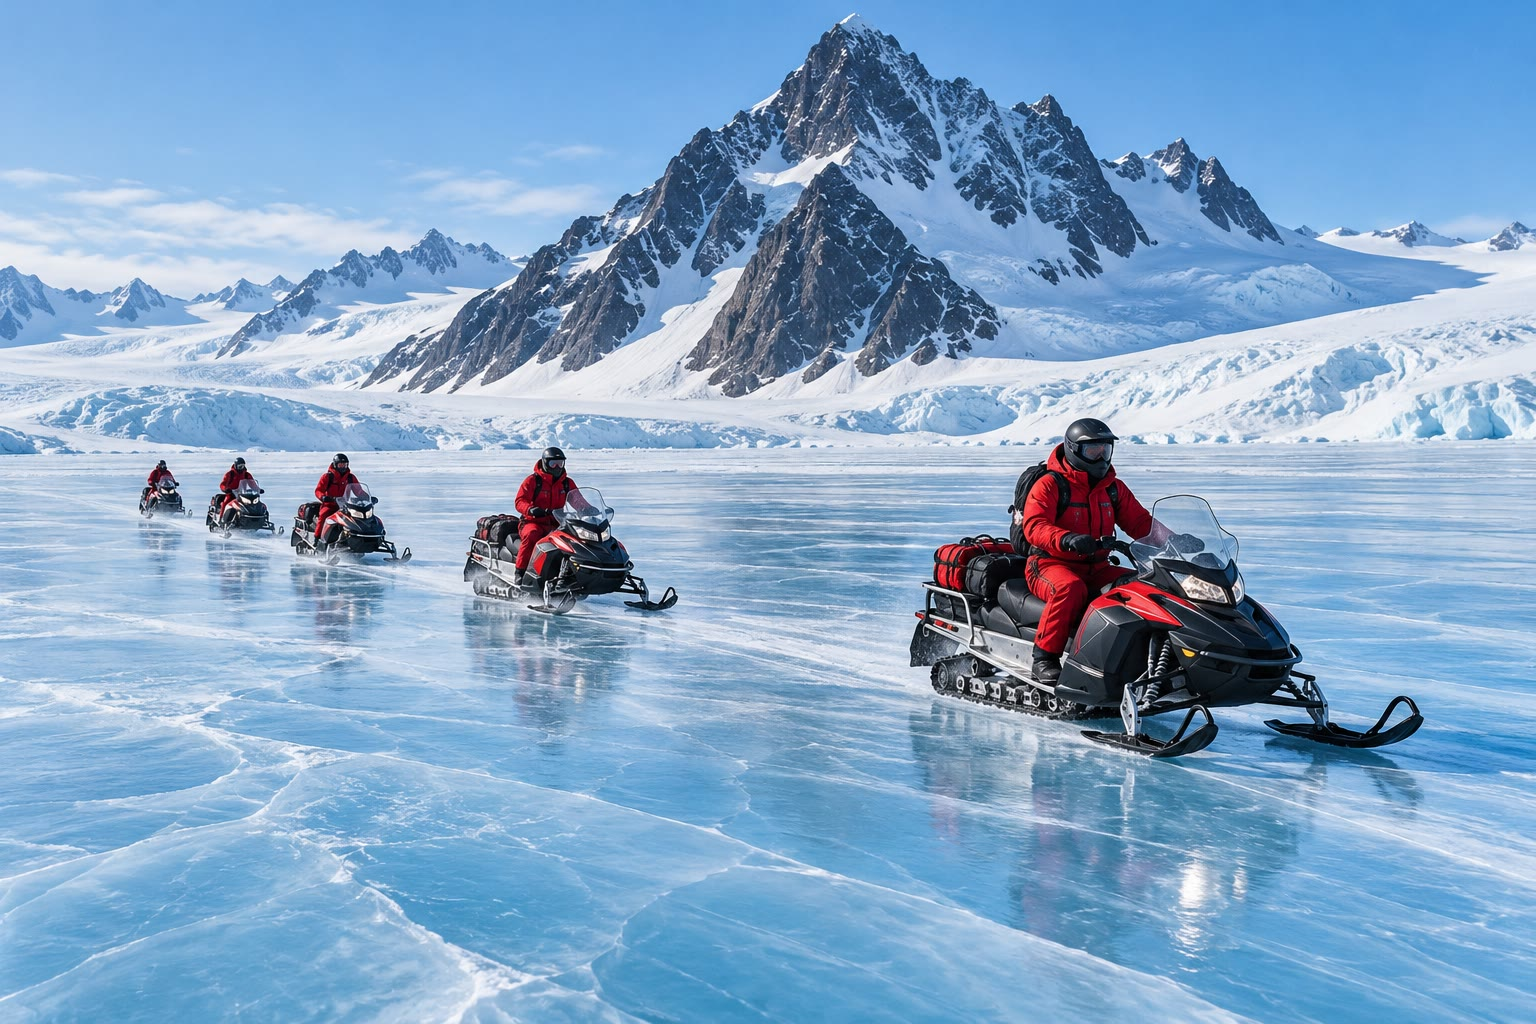
\includegraphics[width=\linewidth]{images/book4/ai/b2-blue-ice-search.jpg}

{\scriptsize 一排搜寻者乘坐雪地摩托，穿过
岩峰下的一片蓝冰平原（AI 生成插图）。}
\end{minipage}
% ledger: folco06:blue-ice, data:b4-meteorites, nasa:antmet
\end{inthefield}

\subsection{球粒陨石}

\begin{definition}[球粒陨石，碳质球粒陨石，陨石球粒，富钙铝包体]
\label{def:b2:planet-formation-meteorites:chondrule}
\emph{球粒陨石}\index{球粒陨石}是一种石质\omterm{def:b2:planet-formation-meteorites:fall-find}{陨石}，其形成后从未熔化过，
且成分除最易挥发的
元素外与太阳接近。其主体由\emph{陨石球粒}\index{陨石球粒}构成，
\omterm{def:b2:planet-formation-meteorites:fall-find}{陨石}球粒是由熔体凝固而成的圆形硅酸盐岩小滴，
直径从十分之一毫米到约一厘米不等，嵌布在
由铁镍金属颗粒和硫化铁组成的细粒基质中。部分球粒\omterm{def:b2:planet-formation-meteorites:fall-find}{陨石}含有
\emph{富钙铝包体}\index{富钙铝包体}（CAI），
即不规则的白色颗粒，主要由钙、铝和钛的矿物组成，
是星云中最早凝聚的产物。
\emph{碳质球粒陨石}\index{碳质球粒陨石}是富含碳、含水矿物和基质的球粒\omterm{def:b2:planet-formation-meteorites:fall-find}{陨石}，
其挥发性元素含量
最接近太阳。
\end{definition}

\omterm{def:b2:planet-formation-meteorites:chondrule}{陨石球粒}仅熔融了数分钟，并在数小时至数天内冷却：星云中某种短暂的局部闪烁加热，
其成因至今未知，熔化了尘埃团块，这些团块凝固成小滴后，
才与尘埃和金属一道聚集成\omterm{def:b2:planet-formation-meteorites:planetesimal}{星子}。
在最原始的\omterm{def:b2:planet-formation-meteorites:fall-find}{陨石}中，\omterm{def:b2:planet-formation-meteorites:chondrule}{陨石球粒}可占其体积的 \qty{90}{\percent}。
\omterm{def:b2:planet-formation-meteorites:chondrule}{富钙铝包体}在普通\omterm{def:b2:planet-formation-meteorites:chondrule}{球粒陨石}中所占比例不到 \qty{1}{\percent}，
在某些\omterm{def:b2:planet-formation-meteorites:chondrule}{碳质球粒陨石}中则超过 \qty{10}{\percent}，
它们形成的时间彼此相差在约十万年以内。
% ledger: gail:meteorites, cy10:growth, cy10:chondrules, gail:chondrite-table, lugaro:cai

\begin{omfigure}
\begin{minipage}[c]{0.5\linewidth}
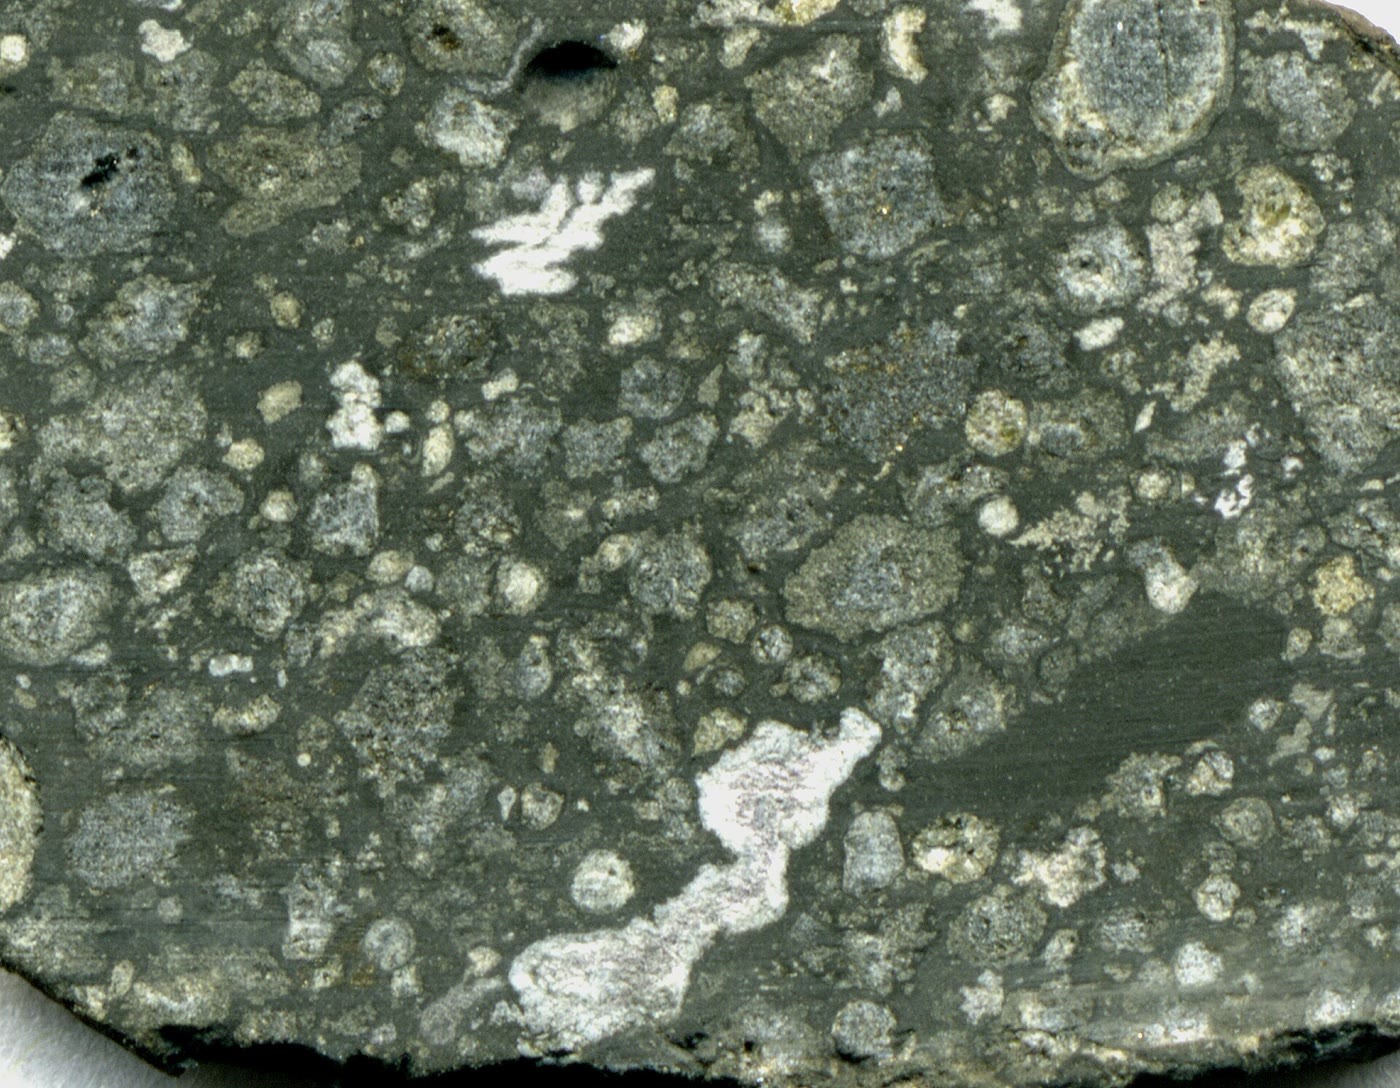
\includegraphics[width=\linewidth]{images/book4/b2-allende-chondrite.jpg}
\end{minipage}\hfill
\begin{minipage}[c]{0.46\linewidth}
{\small 阿连德\omterm{def:b2:planet-formation-meteorites:chondrule}{碳质球粒陨石}（CV3 类）的切面，该\omterm{def:b2:planet-formation-meteorites:fall-find}{陨石}于 1969 年坠落于墨西哥北部，
共收集到约两吨。圆形灰色颗粒为\omterm{def:b2:planet-formation-meteorites:chondrule}{陨石球粒}，不规则白色斑块为\omterm{def:b2:planet-formation-meteorites:chondrule}{富钙铝包体}，深色胶结物为基质。
视野宽约数厘米。
照片：James St.\ John, CC BY 2.0。}
\end{minipage}
% ledger: data:b4-meteorites, gail:chondrite-table
\end{omfigure}

\omterm{def:b2:planet-formation-meteorites:chondrule}{球粒陨石}可分为若干群，它们的差别体现在\omterm{def:b2:planet-formation-meteorites:chondrule}{陨石球粒}的大小与丰度、
金属含量、橄榄石中的铁含量，以及基质所占比例上（见下表）。
普通\omterm{def:b2:planet-formation-meteorites:chondrule}{球粒陨石} H、L 和 LL 群的金属与总铁含量分别为高、低和极低，
其 Fe/Si 原子比分别为
\num{0.80}、\num{0.59} 和 \num{0.53}。
% ledger: gail:chondrite-table

\begin{table}[h]
\centering
\small
\begin{tabular}{lcccccc}
\hline
 & H & L & LL & CI & CM & CV\\
\hline
\omterm{def:b2:planet-formation-meteorites:chondrule}{陨石球粒}（体积\ \%） & 60--80 & 60--80 & 60--80 & $\ll 1$ & 20 & 45\\
平均\omterm{def:b2:planet-formation-meteorites:chondrule}{陨石球粒}直径（mm） & 0.3 & 0.7 & 0.9 &——& 0.3 & 1.0\\
\omterm{def:b2:planet-formation-meteorites:chondrule}{富钙铝包体}（体积\ \%） & 0.1--1 & 0.1--1 & 0.1--1 & $\ll 1$ & 5 & 10\\
基质（体积\ \%） & 10--15 & 10--15 & 10--15 & $> 99$ & 70 & 40\\
铁镍金属（体积\ \%） & 10 & 5 & 2 & 0 & 0.1 & 0--5\\
橄榄石中的铁橄榄石（摩尔 \%） & 16--20 & 23--26 & 27--32 & & & \\
\omterm{def:b2:planet-formation-meteorites:type}{岩石学类型} & 3--6 & 3--6 & 3--6 & 1 & 2 & 3\\
最高温度（K） & 1220 & 1220 & 1220 & 430 & 670 & 870\\
\hline
\end{tabular}
\caption{普通\omterm{def:b2:planet-formation-meteorites:chondrule}{球粒陨石}（H、L、LL）及三个\omterm{def:b2:planet-formation-meteorites:chondrule}{碳质球粒陨石}群的性质。
铁橄榄石：橄榄石的铁端元。数据来源：Gail 等（2014）。}
\label{tab:b2:planet-formation-meteorites:chondrites}
% ledger: gail:chondrite-table
\end{table}

\begin{definition}[岩石学类型]\label{def:b2:planet-formation-meteorites:type}
\omterm{def:b2:planet-formation-meteorites:chondrule}{球粒陨石}的\emph{岩石学类型}\index{岩石学类型}是一个数字，
取值从 1 到 6，记录其母体天体上所经历的变化：类型 3 变化最小；
类型 4 至 6 受热程度逐渐增强，\omterm{def:b2:planet-formation-meteorites:chondrule}{陨石球粒}边界模糊，
矿物重结晶并趋于成分均一；类型 2 和 1 则
受液态水改造逐渐增强，其矿物转变为黏土。
\end{definition}

表格最后一行给出各群达到的最高温度：
最受热的普通\omterm{def:b2:planet-formation-meteorites:chondrule}{球粒陨石}可达约 \qty{1220}{K}，
而 CI \omterm{def:b2:planet-formation-meteorites:chondrule}{球粒陨石}浸泡于水中却从未受热，其最高温度不超过 \qty{430}{K}。
正如上一节所示，这些热量来自母体天体内部。
% ledger: gail:chondrite-table

\subsection{无球粒陨石与铁陨石}

\begin{definition}[无球粒陨石，铁陨石，石铁陨石]
\label{def:b2:planet-formation-meteorites:classes}
\emph{无球粒陨石}\index{无球粒陨石}是一种石质\omterm{def:b2:planet-formation-meteorites:fall-find}{陨石}，它从熔体中结晶，
或在一个曾经熔化的天体中于高温下重结晶，
因此不含球粒。\emph{铁陨石}\index{铁陨石}主要由
铁镍金属构成。\emph{石铁陨石}\index{石铁陨石}
由金属和硅酸盐大致
等量组成。
\end{definition}

这些都是熔化并分异的天体的碎片：\omterm{def:b2:planet-formation-meteorites:classes}{无球粒陨石}是其地壳和地幔，
\omterm{def:b2:planet-formation-meteorites:classes}{铁陨石}是其金属地核，\omterm{def:b2:planet-formation-meteorites:classes}{石铁陨石}则来自金属与硅酸盐相遇之处。
最大的一类\omterm{def:b2:planet-formation-meteorites:classes}{无球粒陨石}是霍华德石、古铜辉\omterm{def:b2:planet-formation-meteorites:classes}{无球粒陨石}和顽火辉石\omterm{def:b2:planet-formation-meteorites:classes}{无球粒陨石}（HED），
它们由玄武岩和富辉石岩石构成，
占全部坠落\omterm{def:b2:planet-formation-meteorites:fall-find}{陨石}的 \qty{5.5}{\percent}。其来源依据光谱和轨道，
被追溯到小行星灶神星，该星直径约 \qty{525}{km}。黎明号探测器
于 2011 年抵达灶神星，证实了这一结论：灶神星表面的化学成分和矿物组成
与 HED \omterm{def:b2:planet-formation-meteorites:fall-find}{陨石}相符，其南极附近一个宽 \qty{500}{km} 的盆地标示出碎片被撞离之处，
其重力场则指示出一个直径约 \qty{225}{km} 的铁质地核。灶神星在其早期历史中
几乎或完全熔化过。
其他\omterm{def:b2:planet-formation-meteorites:classes}{无球粒陨石}来自月球和火星。
收藏中的\omterm{def:b2:planet-formation-meteorites:fall-find}{陨石}似乎来自
约一百个不同的母体天体。
% ledger: data:b4-meteorites, nasa:vesta-dawn, gail:meteorites

\omterm{def:b2:planet-formation-meteorites:classes}{铁陨石}记录了其地核如何冷却。切开并经酸蚀的
断面上可见交错的板片结构（见下图）：高温时金属为铁镍单一合金；
缓慢冷却时，贫镍合金沿原晶体的晶面成板状生长，
冷却越慢，板片越宽。
测量大量\omterm{def:b2:planet-formation-meteorites:classes}{铁陨石}的板片宽度，
即可推得其来源地核的冷却速率。
% ledger: gail:meteorites

\begin{omfigure}
\begin{minipage}[c]{0.5\linewidth}
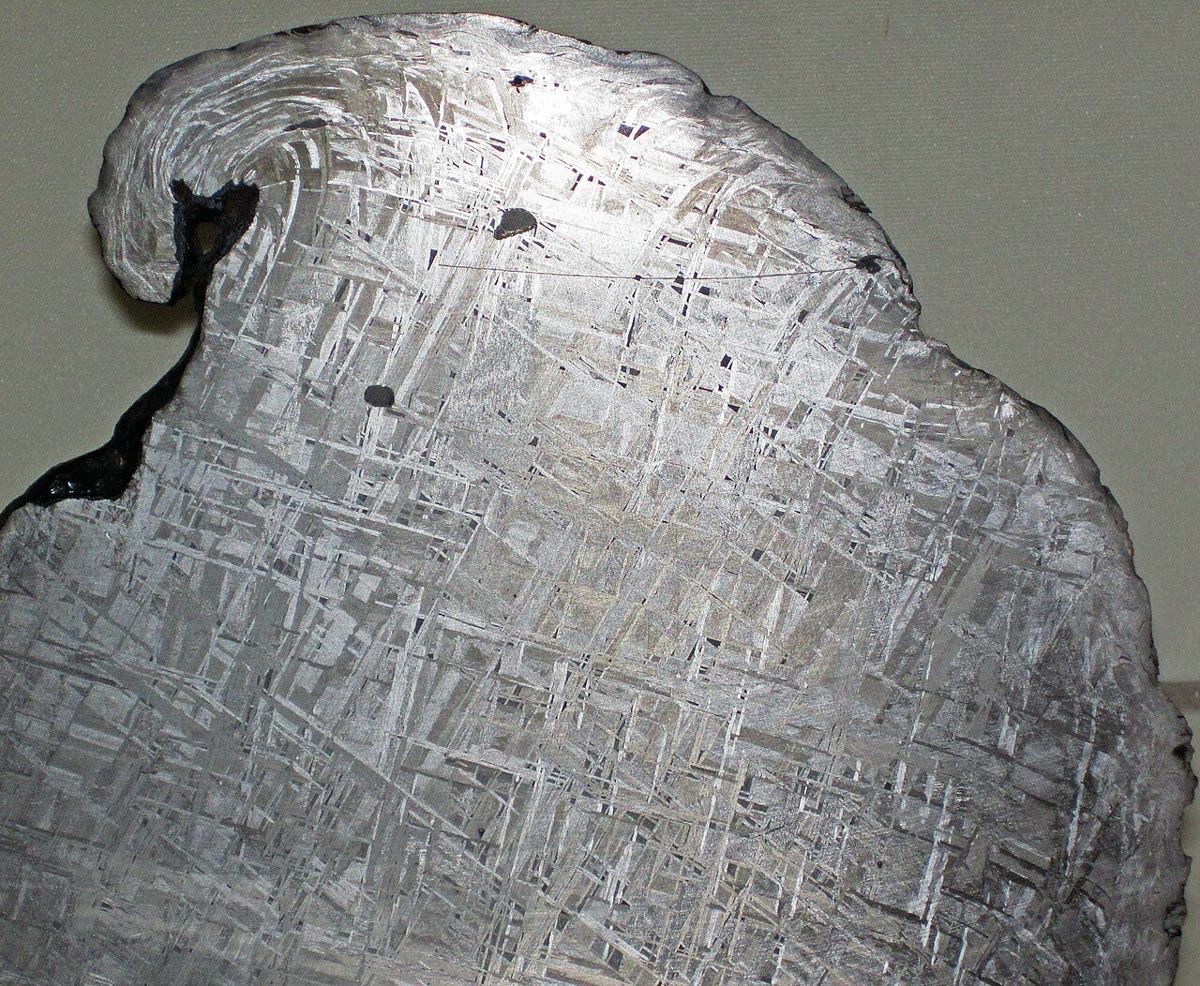
\includegraphics[width=\linewidth]{images/book4/b2-gibeon-widmanstatten.jpg}
\end{minipage}\hfill
\begin{minipage}[c]{0.46\linewidth}
{\small 吉贝恩\omterm{def:b2:planet-formation-meteorites:classes}{铁陨石}一块经切割、抛光并酸蚀的断面，该\omterm{def:b2:planet-formation-meteorites:fall-find}{陨石}发现于纳米比亚：
铁镍合金交错的板片结构（魏德曼施塔滕图样）是其母体天体的金属地核缓慢冷却时形成的。
James St.\ John，
CC BY 2.0。}
\end{minipage}
% ledger: data:b4-meteorites
\end{omfigure}

\section{太阳系的年龄测定}

太阳系的年龄即其最古老固体的年龄。CAI 的铀–铅等时线
依据本科一年级分册中的方法构造，给出 \qtyrange{4567}{4568}{\Ma}；
CAI 彼此形成的时间相差不超过约 \qty{0.1}{Ma}，
这一时间足够短，可将其年龄取为太阳诞生的时刻。
此后几百万年内发生的事件，包括球粒的形成以及首批天体的组装与熔化，
最好相对于 CAI 来定年，
所用“时钟”走得快、停得早。
% ledger: lugaro:cai

\begin{definition}[短寿命放射性核素]
\label{def:b2:planet-formation-meteorites:slr}
称\emph{短寿命放射性核素}\index{短寿命放射性核素}为
半衰期大致在 \num{0.1} 至 \qty{100}{Ma} 之间的放射性核素，
其在太阳系形成时存在、现已灭绝，其曾经存在的痕迹表现为
子体过量，见于富含其母
元素的矿物中。
\end{definition}

最著名的是铝-26，它衰变为镁-26，半衰期为
\qty{0.717}{Ma}（平均寿命为 \qty{1.035}{Ma}）。CAI 形成时，
约每 \num{19000} 个铝原子中有一个为铝-26，其比值
$\ce{^{26}Al}/\ce{^{27}Al}$ 为 $(5.23 \pm 0.13)\times10^{-5}$，
即\emph{标准}值。其他短寿命核素的时间跨度更长（
见下表）。
% ledger: lugaro:al26, lugaro:slr-table

\begin{table}[h]
\centering
\small
\begin{tabular}{lllcc}
\hline
核素 & 子体 & 参考核素 & 半衰期 (Ma) & 早期比值 \\
\hline
\ce{^{26}Al} & \ce{^{26}Mg} & \ce{^{27}Al} & 0.717 & $5.23\times10^{-5}$\\
\ce{^{60}Fe} & \ce{^{60}Ni} & \ce{^{56}Fe} & 2.62 & $1.0\times10^{-8}$\\
\ce{^{53}Mn} & \ce{^{53}Cr} & \ce{^{55}Mn} & 3.74 & $7\times10^{-6}$\\
\ce{^{107}Pd} & \ce{^{107}Ag} & \ce{^{108}Pd} & 6.5 & $6.6\times10^{-5}$\\
\ce{^{182}Hf} & \ce{^{182}W} & \ce{^{180}Hf} & 8.90 & $1.02\times10^{-4}$\\
\ce{^{129}I} & \ce{^{129}Xe} & \ce{^{127}I} & 15.7 & $1.28\times10^{-4}$\\
\hline
\end{tabular}
\caption{太阳系早期的若干\omterm{def:b2:planet-formation-meteorites:slr}{短寿命放射性核素}，列出其稳定子体、
所用作参照的同种元素稳定同位素、其半衰期，以及 CAI 形成时其与参考核素的比值。
数据来自 Lugaro 等人
（2018）。}
\label{tab:b2:planet-formation-meteorites:slr}
% ledger: lugaro:al26, lugaro:slr-table
\end{table}

\begin{proposition}[由已灭绝核素得到的相对年龄]
\label{prop:b2:planet-formation-meteorites:relative-age}
若某短寿命核素与其参考同位素的比值在 CAI 形成时处处为 $R_0$，
而在某天体形成时测得其比值为 $R$，
则该天体形成于
\[
  \Delta t = \tau \ln\frac{R_0}{R}
\]
CAI 之后，其中 $\tau$ 为该核素的平均寿命。
$\delta R$ 为 $R$ 的误差时，$\tau\,\delta R/R$ 即为 $\Delta t$ 的误差。
\end{proposition}

\begin{proof}
参考同位素稳定，因此该比值与放射性核素本身
一样按同样规律衰减：$R = R_0 e^{-\Delta t/\tau}$。取对数，
得 $\Delta t = \tau\ln(R_0/R)$。求微分，$\mathrm d(\Delta t) =
-\tau\,\mathrm dR/R$。
\end{proof}

比值的相对误差为 \qty{10}{\percent} 时，相应的时间误差对铝-26 为 \qty{0.1}{Ma}，
对锰-53 为 \qty{0.54}{Ma}，对铪-182 为 \qty{1.3}{Ma}。由此可见，每种“时钟”
仅在其自身平均寿命的若干倍范围内精确，
故应依事件选取合适的时钟。天体中的比值 $R$
由其矿物读取。
% ledger: lugaro:al26, lugaro:slr-table

\begin{proposition}[铝–镁等时线]
\label{prop:b2:planet-formation-meteorites:al-mg}
设某天体的若干矿物在时刻 $\Delta t$ 同时形成，
具有相同的镁同位素组成 $(\ce{^{26}Mg}/\ce{^{24}Mg})_0$，
但 $\ce{^{27}Al}/\ce{^{24}Mg}$ 各不相同，此后保持封闭。今天，它们
位于如下直线上：
\[
  \frac{\ce{^{26}Mg}}{\ce{^{24}Mg}}
  = \left(\frac{\ce{^{26}Mg}}{\ce{^{24}Mg}}\right)_0
  + R\,\frac{\ce{^{27}Al}}{\ce{^{24}Mg}},
\]
其斜率即为该天体
形成时的比值 $R = \ce{^{26}Al}/\ce{^{27}Al}$。
\end{proposition}

\begin{proof}
形成时存在的每个铝-26 原子，此后都已变成
一个镁-26 原子，因此某矿物获得了
$\ce{^{26}Al}_{\text{当时}} = R\,\ce{^{27}Al}$ 个镁-26 原子，
铝-27 是稳定的。以未变的镁-24 原子数相除，
即得该直线。
\end{proof}

富铝贫镁矿物（如斜长石）显示出大量
过剩的镁-26；几乎不含铝的橄榄石则完全没有。这就是
早期太阳系时间序列的建立过程：\omterm{def:b2:planet-formation-meteorites:chondrule}{富钙铝包体}（CAI）最早；球粒
随后几百万年间形成，球粒的证据将气盘寿命限定为
不足五百万年；\omterm{def:b2:planet-formation-meteorites:chondrule}{球粒陨石}的母体
在其最年轻的球粒形成之后才聚集。狄奥根尼特
是灶神星地幔的岩石，在 CAI 形成后约一百万年内开始结晶，
灶神星的地核形成于最初的一至
四百万年之内；\omterm{def:b2:planet-formation-meteorites:classes}{铁陨石}和\omterm{def:b2:planet-formation-meteorites:classes}{无球粒陨石}比许多
\omterm{def:b2:planet-formation-meteorites:chondrule}{球粒陨石}更古老。
% ledger: lugaro:cai, gail:vesta, gail:meteorites

\section{铝-26 的热量与最初的熔化}

熔化灶神星并使普通
\omterm{def:b2:planet-formation-meteorites:chondrule}{球粒陨石}变质的热量从何而来？模型与\omterm{def:b2:planet-formation-meteorites:fall-find}{陨石}研究一致表明，在最早的天体中，
主要热源是铝-26 的衰变。\omterm{def:b2:planet-formation-meteorites:chondrule}{球粒陨石}成分的岩石起初携带
每千克 \qty{5}{MJ}，可在几百万年内释放：
若热量无法逸出，足以使岩石升温数千开尔文。
% ledger: lugaro:heat, lugaro:melting

\begin{proposition}[铝-26 对星子的加热]
\label{prop:b2:planet-formation-meteorites:heating}
设岩石每千克接收放射性功率 $H_0 e^{-t/\tau}$，
比热容为 $c$ 且不失热，则其在吸积时刻
$t_a$ 之后按下式升温：
\[
  T(t) = T_0 + \frac{H_0\tau}{c}\left(e^{-t_a/\tau} - e^{-t/\tau}\right),
\]
并趋于峰值温度
$T_{\max} = T_0 + (H_0\tau/c)\,e^{-t_a/\tau}$。临界温度
$T_c > T_0$ 仅当天体吸积于下式所示时刻之前时才能达到：
\[
  t_a^* = \tau\ln\frac{H_0\tau}{c\,(T_c - T_0)}.
\]
\end{proposition}

\begin{proof}
不计热损失，$c\,\mathrm dT/\mathrm dt = H_0 e^{-t/\tau}$。从
$t_a$ 积分，此时 $T = T_0$，得
$c\,(T - T_0) = H_0\tau\,(e^{-t_a/\tau} - e^{-t/\tau})$，它趋于
$H_0\tau e^{-t_a/\tau}$，当 $t \to \infty$ 时。令 $T_{\max} = T_c$，并求解
$t_a$ 得 $t_a^*$；吸积越早，峰值越高。
\end{proof}

普通\omterm{def:b2:planet-formation-meteorites:chondrule}{球粒陨石}母体的一个模型取
$H_0 = \qty{1.9e-7}{W.kg^{-1}}$，$c = \qty{837}{J.kg^{-1}.K^{-1}}$ 及
$T_0 = \qty{250}{K}$。于是 $H_0\tau/c$ 约为 \qty{7400}{K}。三个
温度值得注意：约 \qty{750}{K} 时，多孔岩石开始烧结成
致密岩石；约 \qty{1200}{K} 时，金属与硫化铁开始共同熔化；
约 \qty{1700}{K} 时最后的硅酸盐熔化。吸积时间早于
\qty{1.7}{Ma} 的天体完全熔化；早于 \qty{2.1}{Ma} 的，其金属与硫化物
熔化并可下沉形成地核；直至约 \qty{2.8}{Ma}，它至少已
烧结并变质；更晚形成的天体则保持低温（见下图）。
% ledger: gail:params, gail:temps, lugaro:al26

\begin{omfigure}
\begin{tikzpicture}
\begin{axis}[omrecord, name=left, width=0.45\linewidth, height=6.0cm,
  xmin=0, xmax=8, ymin=0, ymax=2300,
  xlabel={CAI 之后的时间 (Ma)}, ylabel={温度 (K)},
  tick label style={font=\scriptsize}, label style={font=\small}]
\addplot[black!45, densely dashed, domain=0:8, samples=2] {750};
\addplot[black!45, densely dashed, domain=0:8, samples=2] {1200};
\addplot[black!45, densely dashed, domain=0:8, samples=2] {1700};
\addplot[thick, red!75!black] table[x=t_Myr, y=T_K] {figdata/out/bachelor-2-al26-ta15.dat};
\addplot[thick, orange!80!black] table[x=t_Myr, y=T_K] {figdata/out/bachelor-2-al26-ta20.dat};
\addplot[thick, teal!70!black] table[x=t_Myr, y=T_K] {figdata/out/bachelor-2-al26-ta25.dat};
\addplot[thick, blue!70!black] table[x=t_Myr, y=T_K] {figdata/out/bachelor-2-al26-ta30.dat};
\node[font=\tiny, red!75!black, anchor=south east] at (axis cs:7.9,1995) {$t_a = \qty{1.5}{Ma}$};
\node[font=\tiny, orange!80!black, anchor=south east] at (axis cs:7.9,1325) {2};
\node[font=\tiny, teal!70!black, anchor=south east] at (axis cs:7.9,915) {2.5};
\node[font=\tiny, blue!70!black, anchor=north east] at (axis cs:7.9,650) {3};
\node[font=\tiny, black!60, anchor=south west] at (axis cs:0.1,1700) {硅酸盐熔化};
\node[font=\tiny, black!60, anchor=south west] at (axis cs:0.1,1200) {Fe--FeS 熔化};
\node[font=\tiny, black!60, anchor=south west] at (axis cs:0.1,750) {烧结};
\end{axis}
\begin{axis}[omrecord, at={(left.east)}, anchor=west, xshift=2.1cm, width=0.45\linewidth,
  height=6.0cm, xmin=0, xmax=4, ymin=0, ymax=8000,
  xlabel={吸积时间 $t_a$ (Ma)}, ylabel={峰值温度 (K)},
  tick label style={font=\scriptsize}, label style={font=\small},
  scaled y ticks=false, yticklabel style={/pgf/number format/1000 sep={\,}}]
\addplot[black!45, densely dashed, domain=0:4, samples=2] {750};
\addplot[black!45, densely dashed, domain=0:4, samples=2] {1200};
\addplot[black!45, densely dashed, domain=0:4, samples=2] {1700};
\addplot[thick, black] table[x=ta_Myr, y=Tpeak_K] {figdata/out/bachelor-2-al26-peak.dat};
\draw[black!60] (axis cs:1.69,0) -- (axis cs:1.69,1700);
\draw[black!60] (axis cs:2.13,0) -- (axis cs:2.13,1200);
\node[font=\tiny, black!70, anchor=south] at (axis cs:2.0,4500) {\qty{1.7}{Ma}};
\draw[black!50, -latex] (axis cs:2.0,4450) -- (axis cs:1.71,1800);
\node[font=\tiny, black!70, anchor=south] at (axis cs:2.9,3300) {\qty{2.1}{Ma}};
\draw[black!50, -latex] (axis cs:2.9,3250) -- (axis cs:2.16,1300);
\end{axis}
\end{tikzpicture}

\par\smallskip{\small 铝-26 对无热损失的\omterm{def:b2:planet-formation-meteorites:chondrule}{球粒陨石}质天体内部的加热
（上述命题；$H_0 = \qty{1.9e-7}{W.kg^{-1}}$，
$c = \qty{837}{J.kg^{-1}.K^{-1}}$，$T_0 = \qty{250}{K}$，$\tau = \qty{1.035}{Ma}$）。
左图：吸积于 CAI 之后 1.5、2、2.5 及 \qty{3}{Ma} 的天体，其温度
随时间的变化。右图：峰值温度随吸积时间的变化，
吸积早于 \qty{1.7}{Ma} 的天体熔化，早于 \qty{2.1}{Ma} 的，其金属与硫化物熔化。
真实天体会把部分热量用于熔化，从而限制温度上升，并在
近表面散失热量。模型数值：Gail 等（2014）。}
% ledger: gail:params, gail:temps, lugaro:al26
\end{omfigure}

该命题忽略了热量散失，这一近似只在大天体的深部成立。
热量扩散的距离为 $\sqrt{\kappa t}$，时间为 $t$，其中
$\kappa$ 为岩石的热扩散率：取模型的数值，
在铝-26 的一个平均寿命内，热量扩散的距离约为 \qty{5}{km}（见\cref{exo:b2:planet-formation-meteorites:12}）。
远小于此的天体，其热量散失的速度与产生热量的速度相当；详细的
模型表明，直径超过 \qtyrange{10}{20}{km} 的天体可能发生熔化。
% ledger: gail:params, lugaro:melting

\begin{definition}[行星分异]
\label{def:b2:planet-formation-meteorites:differentiation}
\emph{行星分异}\index{行星分异}是指天体在熔融或部分熔融之后，
按成分与密度分成不同层次的过程，即
金属地核、硅酸盐地幔，以及
由最后熔体形成的地壳。
\end{definition}

\omterm{def:b2:planet-formation-meteorites:fall-find}{陨石}因此记录了两类早期天体。形成于最初约两百万年内的天体
所含铝-26 足以使其熔化并
发生分异：地核为\omterm{def:b2:planet-formation-meteorites:classes}{铁陨石}，地壳和地幔为
\omterm{def:b2:planet-formation-meteorites:classes}{无球粒陨石}，灶神星则是唯一的幸存者。此后形成的天体
仍为\omterm{def:b2:planet-formation-meteorites:chondrule}{球粒陨石}，其内部加热程度取决于形成时间，
也取决于各碎片所处的深度：最深的成为 6 型，最浅的仍为
3 型。地球本身由两类天体的胚胎与\omterm{def:b2:planet-formation-meteorites:planetesimal}{星子}聚集而成，
并经历巨大撞击，分异为地核、地幔和地壳。
% ledger: gail:meteorites, gail:vesta, gail:temps

\section{练习}

\begin{exercise}[$\star$]\label{exo:b2:planet-formation-meteorites:1}
在最小质量\omterm{def:b2:planet-formation-meteorites:nebula}{太阳星云}中，计算气体在 \qty{1}{au} 和 \qty{5.2}{au} 处的面密度，
以及固体在 \qty{1}{au} 和 \qty{5.2}{au} 处的面密度：
在 \qty{1}{au} 处仅计岩石（$Z_{\mathrm{rel}} = 0.33$），
在 \qty{5.2}{au} 处所有冰均已凝结（$Z_{\mathrm{rel}} = 1$）。
在 \qty{5.2}{au} 处，气体的面密度是固体的多少倍？
% ledger: cy10:mmsn
\end{exercise}

\begin{exercise}[$\star$]\label{exo:b2:planet-formation-meteorites:2}
利用凝结温度图，将铝、钠、镁、铁、硫和氧（以水冰计）
按凝结先后排序，并给出每种元素的挥发性组别。
其中哪些元素预计在 CAI 中富集，
相对于太阳，哪些在地球中贫化？
% ledger: lodders:tc-table, lodders:groups
\end{exercise}

\begin{exercise}[$\star$]\label{exo:b2:planet-formation-meteorites:3}
该目录列出 \num{1107} 块\omterm{def:b2:planet-formation-meteorites:fall-find}{陨石}目击坠落，其中 856 块为普通\omterm{def:b2:planet-formation-meteorites:chondrule}{球粒陨石}，
49 块为\omterm{def:b2:planet-formation-meteorites:classes}{铁陨石}；另有 \num{44534} 块\omterm{def:b2:planet-formation-meteorites:fall-find}{发现型陨石}，其中 \num{38647} 块为普通\omterm{def:b2:planet-formation-meteorites:chondrule}{球粒陨石}，
\num{1020} 块为\omterm{def:b2:planet-formation-meteorites:classes}{铁陨石}，\num{22096} 块来自 南纬 \ang{60} 以南。计算
目击坠落\omterm{def:b2:planet-formation-meteorites:fall-find}{陨石}与\omterm{def:b2:planet-formation-meteorites:fall-find}{发现型陨石}中普通\omterm{def:b2:planet-formation-meteorites:chondrule}{球粒陨石}和\omterm{def:b2:planet-formation-meteorites:classes}{铁陨石}所占的比例，
以及南极\omterm{def:b2:planet-formation-meteorites:fall-find}{发现型陨石}所占的比例。若要估计各类\omterm{def:b2:planet-formation-meteorites:fall-find}{陨石}到达地球的比例，
你会使用哪一类样本？请说明理由。
% ledger: data:b4-meteorites
\end{exercise}

\begin{exercise}[$\star$]\label{exo:b2:planet-formation-meteorites:4}
某天体矿物给出的初始比值为
$\ce{^{26}Al}/\ce{^{27}Al} = \num{1.0e-5}$。该天体在 CAI 形成之后多久形成？
取 $R_0 = \num{5.23e-5}$，平均寿命为 \qty{1.035}{Ma}。
% ledger: lugaro:al26
\end{exercise}

\begin{exercise}[$\star\star$]\label{exo:b2:planet-formation-meteorites:5}
利用\cref{prop:b2:planet-formation-meteorites:disc-mass}，取
\qty{1}{au} 处 $\Sigma_1 = \qty{2.2e4}{kg.m^{-2}}$（\qty{1}{au} $=
\qty{1.496e11}{m}$，$M_\odot = \qty{1.989e30}{kg}$），计算最小质量星云
在 \qty{30}{au} 以内和 \qty{100}{au} 以内的质量，以太阳质量为单位，
并与观测到的盘（质量为 \numrange{0.001}{0.1} 个太阳质量）进行比较。
% ledger: cy10:mmsn
\end{exercise}

\begin{exercise}[$\star\star$]\label{exo:b2:planet-formation-meteorites:6}
在被动盘 $T = \qty{120}{K}\,(r/\qty{1}{au})^{-3/7}$ 中，求水冰
（\qty{182}{K}）和甲烷冰（\qty{41}{K}）稳定存在的位置。直射阳光下的尘粒
在 \qty{2.3}{au} 处达到 \qty{182}{K}。为何两种\omterm{def:b2:planet-formation-meteorites:snow-line}{雪线}位置的估计
不相同？哪一种适用于构成行星的天体？
% ledger: cy10:passive, lodders:phases
\end{exercise}

\begin{exercise}[$\star\star$]\label{exo:b2:planet-formation-meteorites:7}
取 $b = 5$，计算最小质量星云中位于 \qty{1}{au} 处的胚胎
（$\Sigma_p = \qty{10.9}{g.cm^{-2}}$）以及位于\omterm{def:b2:planet-formation-meteorites:snow-line}{雪线}之外的胚胎
（\qty{5.2}{au} 处，$\Sigma_p = \qty{2.78}{g.cm^{-2}}$）的隔离质量，以地球质量为单位，
（$M_\oplus = \qty{5.972e24}{kg}$，$M_\odot = \qty{1.989e30}{kg}$）。
若在 \qty{5.2}{au} 处的盘中固体物质多出 \num{3.5} 倍，它会变成多少？
% ledger: cy10:isolation, cy10:mmsn, earth:mass
\end{exercise}

\begin{exercise}[$\star\star$]\label{exo:b2:planet-formation-meteorites:8}
CI 成分的岩石在 CAI 形成时，每克含有 \num{1.01e16} 个铝-26 原子，
每次衰变释放 \qty{5.00e-13}{J} 的热量。计算
整个衰变过程中每千克岩石释放的热量，以及
在 $c = \qty{837}{J.kg^{-1}.K^{-1}}$ 且无热损失的条件下它所引起的温升。
该热量是将岩石从 \num{250} 加热到
\qty{1700}{K} 所需热量的多少倍？
% ledger: lugaro:heat, gail:params
\end{exercise}

\begin{exercise}[$\star\star$]\label{exo:b2:planet-formation-meteorites:9}
铝-26 在整个衰变过程中，每克 CI 岩石释放 \qty{5.07e10}{erg}；
铁-60 则每克释放 \qty{7.49e7}{erg}。计算两者释放能量之比。
铁-60 的半衰期为 \qty{2.62}{Ma}：计算其平均寿命，
以及两者的初始加热功率之比（能量除以平均寿命）。
% ledger: lugaro:heat, lugaro:slr-table, lugaro:al26
\end{exercise}

\begin{exercise}[$\star\star\star$]\label{exo:b2:planet-formation-meteorites:10}
利用\cref{exo:b2:planet-formation-meteorites:9}的结果，求出铁-60 加热岩石
的速率超过铝-26 的时刻。若某天体在该时刻之后才吸积，铁-60 能否使其熔化？
（请将此时仍需释放的能量与将岩石从 \num{250} 加热到 \qty{1700}{K}
所需的 \qty{1.2e6}{J.kg^{-1}} 进行比较。）
% ledger: lugaro:heat, lugaro:slr-table, lugaro:al26
\end{exercise}

\begin{exercise}[$\star\star\star$]\label{exo:b2:planet-formation-meteorites:11}
已知 $H_0 = \qty{1.9e-7}{W.kg^{-1}}$，$\tau = \qty{1.035}{Ma}$，
$c = \qty{837}{J.kg^{-1}.K^{-1}}$ 和 $T_0 = \qty{250}{K}$（一年为
\qty{3.156e7}{s}），求使大型天体中心分别达到
\qty{1200}{K} 和 \qty{1700}{K} 的最晚吸积时刻。部分测量表明，
盘的部分区域中初始铝-26 仅为标准值的一半：
两个时刻各会移动多少？证明该移动量
与临界温度无关。
% ledger: gail:params, gail:temps, lugaro:al26
\end{exercise}

\begin{exercise}[$\star\star\star$]\label{exo:b2:planet-formation-meteorites:12}
岩石的传导率为 \qty{2.1}{W.m^{-1}.K^{-1}}，密度为
\qty{3300}{kg.m^{-3}}，比热容为 \qty{837}{J.kg^{-1}.K^{-1}}，其
热扩散率为 $\kappa = k/(\rho c)$。求其值，以及
铝-26 一个平均寿命内热量扩散的距离 $\sqrt{\kappa\tau}$。
试说明加热命题为何适用于直径为
\qty{100}{km} 的天体中心，而不适用于直径为 \qty{2}{km} 的天体，并
与直径为 \qtyrange{10}{20}{km} 的能够熔化的最小天体进行比较。
% ledger: gail:params, lugaro:melting, lugaro:al26
\end{exercise}

\section{问题：落在冰封湖上的石头}

\begin{problem}[{周末问题——对新近坠落的石块进行分类，
用铝-26 测定其陨石球粒的年代，并求出其母体曾达到多高的温度}]
\label{pb:b2:planet-formation-meteorites:1}
% values: calc/ch02.py
% ledger: data:b4-meteorites, gail:chondrite-table, lugaro:al26, lugaro:cai, gail:params, gail:temps, cy10:mmsn, cy10:isolation, lodders:tc-table, earth:mass
冬夜，一颗火流星划过一座虚构的北方湖泊上空，
并伴有巨响。次日清晨，一块 \qty{2.4}{kg}、表面覆黑色熔壳的石块
被拾起于冰面上，位于积雪中一处新鲜火山口的中央。
切开的石块中，\omterm{def:b2:planet-formation-meteorites:chondrule}{陨石球粒}占其体积的 \qty{75}{\percent}，平均
直径为 \qty{0.3}{mm}，边界模糊；金属占其体积的 \qty{9}{\percent}，
其橄榄石中铁橄榄石的摩尔百分比为 18\%。
某实验室分析了一颗\omterm{def:b2:planet-formation-meteorites:chondrule}{陨石球粒}（见下表）。请利用本章的表格，
并取 $R_0 = \num{5.23e-5}$，$\tau = \qty{1.035}{Ma}$，一年为 \qty{3.156e7}{s}，
$H_0 = \qty{1.9e-7}{W.kg^{-1}}$，$c = \qty{837}{J.kg^{-1}.K^{-1}}$，
$T_0 = \qty{250}{K}$，传导率为 \qty{2.1}{W.m^{-1}.K^{-1}}，密度为
\qty{3300}{kg.m^{-3}}，\qty{1}{au} $= \qty{1.496e11}{m}$，
$M_\odot = \qty{1.989e30}{kg}$ 和 $M_\oplus = \qty{5.972e24}{kg}$。

\begin{center}
\small
\begin{tabular}{lcc}
\hline
矿物 & $\ce{^{27}Al}/\ce{^{24}Mg}$ & $\ce{^{26}Mg}/\ce{^{24}Mg}$\\
\hline
橄榄石 & 0.05 & \num{0.139500}\\
玻璃 & 3.00 & \num{0.139518}\\
斜长石 & 15.0 & \num{0.139590}\\
\hline
\end{tabular}
\end{center}

\medskip
\noindent\textbf{第一部分——石块。}
\begin{enumerate}
  \item 该石块是目击陨落还是\omterm{def:b2:planet-formation-meteorites:fall-find}{发现型陨石}？为何这使它具有价值？
  \item 目录中共 \num{1107} 次陨落，其中 856 次为普通\omterm{def:b2:planet-formation-meteorites:chondrule}{球粒陨石}。随机
        抽取一次陨落，它为普通\omterm{def:b2:planet-formation-meteorites:chondrule}{球粒陨石}的概率是多少？
  \item 利用\omterm{def:b2:planet-formation-meteorites:chondrule}{球粒陨石}群表，判断该石块属于哪一群。
  \item 其\omterm{def:b2:planet-formation-meteorites:chondrule}{陨石球粒}边界模糊，矿物成分均一。由此可推断其\omterm{def:b2:planet-formation-meteorites:type}{岩石学类型}，
        并求其所属\omterm{def:b2:planet-formation-meteorites:chondrule}{球粒陨石}群曾达到的最高温度，
        分别以开尔文和摄氏度表示？
  \item 为何预计其中\omterm{def:b2:planet-formation-meteorites:chondrule}{富钙铝包体}较少，而该石块仍比任何
        \omterm{def:b2:planet-formation-meteorites:chondrule}{富钙铝包体}都年轻？
\end{enumerate}

\noindent\textbf{第二部分——球粒形成于何时？}
\begin{enumerate}[resume]
  \item 试说明为何在不同矿物之间，$\ce{^{26}Mg}/\ce{^{24}Mg}$ 比值
        随 $\ce{^{27}Al}/\ce{^{24}Mg}$ 的增大而升高。
  \item 由橄榄石和斜长石的数据，计算等时线的斜率。
        该斜率表示什么？
  \item 验证玻璃的数据点位于同一直线上。
  \item 球粒形成于\omterm{def:b2:planet-formation-meteorites:chondrule}{富钙铝包体}之后多久？
  \item 取\omterm{def:b2:planet-formation-meteorites:chondrule}{富钙铝包体}的年龄为 \qty{4567.5}{\Ma}，求球粒的年龄。
  \item 若某矿物形成于\omterm{def:b2:planet-formation-meteorites:chondrule}{富钙铝包体}之后 
        \qty{10}{Ma}，其中 $\ce{^{26}Al}/\ce{^{27}Al}$ 比值应为多少？表中哪一种核素
        更适合用于测定该事件的年龄？
\end{enumerate}

\noindent\textbf{第三部分——母体的加热。}
该石块的母体半径为 \qty{20}{km}，于\omterm{def:b2:planet-formation-meteorites:chondrule}{富钙铝包体}之后
\qty{2.4}{Ma} 组装而成，紧随其球粒形成之后。
\begin{enumerate}[resume]
  \item 求岩石的热扩散率，以及热量从中心逸出所需的时间 $R^2/\kappa$，
        以百万年计。能否将中心视为
        不散失热量？
  \item 求组装时刻，每千克岩石中铝-26 的
        加热功率。
  \item 求组装之后每千克岩石仍需释放的热量。
  \item 求中心的温升及其峰值温度。
  \item 将结果与本章的三个临界温度比较，中心是否
        熔化？这与第 4 题的结果是否一致？
  \item 中心的金属与硫化物将开始熔化的最晚
        组装时刻是多少？
  \item 组装之后经过多久，温升才达到 \qty{90}{\percent}？
        并给出该时刻相对于\omterm{def:b2:planet-formation-meteorites:chondrule}{富钙铝包体}的年代。
\end{enumerate}

\noindent\textbf{第四部分——邻近天体。}
\begin{enumerate}[resume]
  \item 一块\omterm{def:b2:planet-formation-meteorites:classes}{无球粒陨石}来自某天体，该天体在\omterm{def:b2:planet-formation-meteorites:chondrule}{富钙铝包体}之后
        \qty{0.8}{Ma} 组装完成。求该命题给出的峰值温度，并说明
        该天体实际发生了什么。
  \item 该天体在组装时每千克所含铝-26 为石块母体的
        多少倍？
  \item 该石块的锌与铅含量低于太阳，而镁与
        铝则不然。请利用\omterm{def:b2:planet-formation-meteorites:condensation}{凝聚温度}解释其原因。
  \item 在最小质量\omterm{def:b2:planet-formation-meteorites:nebula}{太阳星云}中，求岩石的面密度
        （$Z_{\mathrm{rel}} = 0.33$）在 \qty{2.5}{au} 处的值，
        该处即母体曾绕行的位置。
  \item 取 $b = 5$，求 \qty{2.5}{au} 处的隔离质量，以千克
        和地球质量表示，并与母体质量进行比较。
  \item 求出母体中心的峰值温度，即本题的关键数值，
        并以摄氏度表示。
\end{enumerate}
\end{problem}
